\chapter{Methodologie}
\todo[inline]{concreet doel?}

Dit hoofdstuk beschrijft hoe de voorgaande theoretische componenten samen een automatische generator van afbeeldingsbeschrijvingen kunnen vormen. De eerste sectie behandelt een bestaande implementatie, die het startpunt vormt van het nieuwe systeem. De volgende secties bekijken uitbreidingen hierop samen met hun implementatie. 

De meeste uitbreidingen hebben als doel om extra semantische informatie aan het taalmodel toe te voegen. Op deze manier blijft het model over kennis beschikken van de originele afbeelding. \todo{Waarom dit nuttig is etc. verdient volgens mij meer aandacht}Eerst volgt een bespreking van hoe het mogelijk is om semantische kennis te extraheren met behulp van LDA. De volgende sectie bespreekt de Flickr30k Entities dataset als een tweede mogelijke bron van informatie. CCA vormt een laatste manier waarin een multimodale vector deze informatie biedt.

Vervolgens beschouwt dit hoofdstuk op welke wijze deze informatie kan bijdragen tot de twee gebruikte taalmodellen. Dit kan als vector rechtstreeks in het RNN of als een semantische gids in het LSTM-netwerk. 

De laatste twee secties bespreken nog twee toevoegingen die geen semantische informatie toevoegen aan het netwerk. De voorlaatste sectie beschrijft een normalisatiemethode voor beam-search. Dit hoofdstuk sluit af met de implementatie van een ander type van neuraal netwerk, dat volgens de auteurs ervan veel veelbelovende eigenschappen heeft.


\section{Startpunt}
Het startpunt van onze implementatie is de code aangereikt door Karpathy op zijn GitHub pagina\footnote{\url{https://github.com/karpathy/neuraltalk}}. Die bevat een Python implementatie van het recurrente neurale netwerk beschreven in zijn paper\cite{Karpathy2015}. Daarnaast bevat het ook een implementatie gebaseerd op het werk van Vinyals et al.\cite{Google}. De idee\"en aangebracht in deze masterproef zijn ge\"implementeerd als extensies van dit startpunt.

\subsection{Algemeen systeem}
Karpathy implementeert beide taalnetwerken zelf en voorziet daarrond een gemeenschappelijk systeem. Dit systeem is verantwoordelijk voor het laden en voorbereiding van de data, het maken van tussentijdse back-ups en het aansturen van een ``oplosser''. Deze ``oplosser'' beheert de netwerken en controleert het trainingsproces. De netwerken worden getraind in batches. Hierbij traint het netwerk niet met steeds \'e\'en voorbeeld, maar met meerdere tegelijk. 
Hij voorziet verschillende opties om dit gemeenschappelijk systeem te configureren. Hieronder volgt een overzicht van de belangrijkste parameters voor het trainen van het netwerk.
\begin{itemize}
	\item Grootte van de verborgen laag van de netwerken
	\item Grootte van afbeeldings- en woordcodering
	\item Aantal afbeeldingen in een batch
	\item Type solver: rmsprop, adagrad, adadelta of vanilla
	\item Decay rate
	\item Al dan niet gradient clipping
	\item Drop-out in encoder en decoder
	\item Leersnelheid
	\item Epsilon smoothing
\end{itemize}
Als CNN gebruikt hij een bestaand vooraf getraind netwerk.

\subsection{Recurrent Neuraal Netwerk}
\label{sec:rnn_methodology}
Een eerste implementatie, die ons startpunt vormt, is beschreven door Karpathy \cite{Karpathy2015}. Hij beschrijft een systeem dat op basis van een afbeelding een beschrijvende zin genereert. Dit gebeurt in twee stappen. Eerst wordt de afbeelding door middel van een CNN omgezet naar een vector representatie. Deze vector dient vervolgens als input voor een recurrent neuraal netwerk dat een grammaticaal correcte beschrijving genereert.

\paragraph{Afbeeldingsrepresentatie}
\label{sec:usedcnn}
Een afbeelding (2D matrix met een RGB waarde voor elke pixel) bevat weinig tastbare informatie. Om dit probleem op te lossen, transformeren de meeste systemen de afbeeldingen eerst naar een vectorrepresentatie. Meestal is deze vector een kansverdeling over verschillende latente concepten uit de afbeelding. De meeste bestudeerde algoritmes maken hiervoor gebruik van een convolutioneel neuraal netwerk (CNN), zoals beschreven in \ref{sec:CNN}.

Het CNN dat momenteel het beste presteert is VGGNet\cite{Arge2015}. Dit netwerk maakt gebruik van 16 lagen, wat veel meer is dan gebruikelijk was op het moment van publicatie. Door het grote aantal lagen kan het netwerk complexere verbanden leren. De lagen bestaan uit groepen van convolutionele lagen afgewisseld met max-pool lagen, zoals beschreven in sectie \ref{sec:CNN}.

De laatste lagen van het netwerk zijn standaard (volledig verbonden) lagen, gevolgd door een softmaxlaag om de output van het netwerk te normaliseren. Figuur \ref{fig:alexvgg} toont een vereenvoudigde weergave van de architectuur van VGGNet, in vergelijking met het vroeger zeer populaire AlexNet\cite{Krizhevsky2012a}.

\begin{figure}[tb]
    \centering
    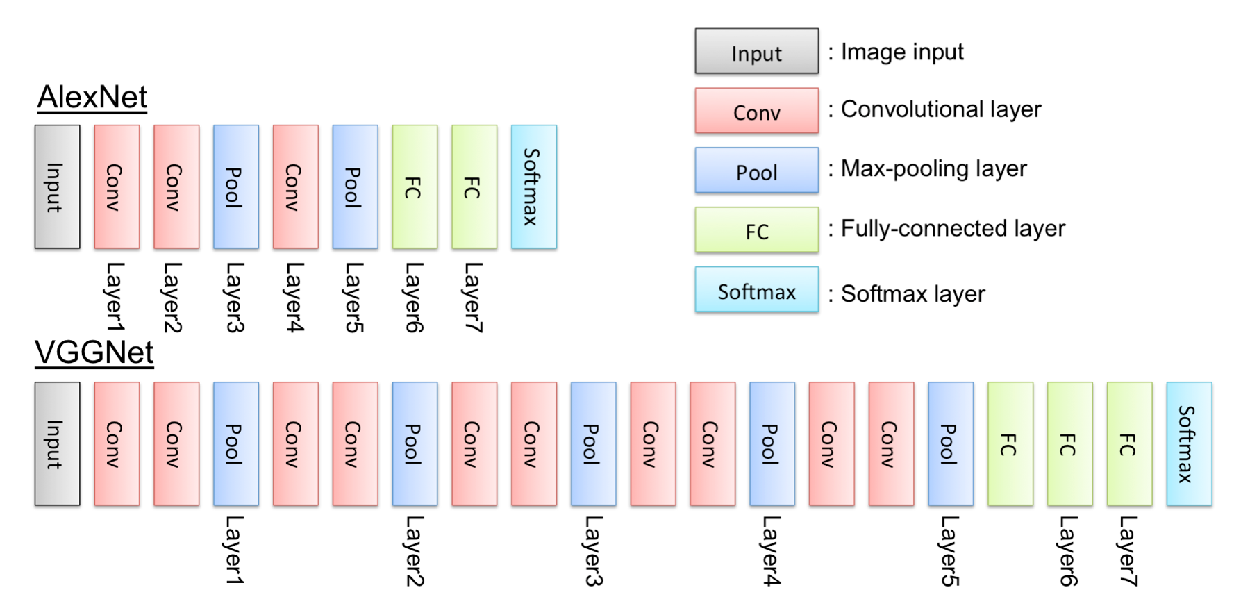
\includegraphics[width=\linewidth]{Images/alex_vgg.eps}
    \caption{Vergelijking van de architectuur van AlexNet en VGGNet}
    \label{fig:alexvgg}
\end{figure}


De representatie die wordt gebruik door Karpathy is de output van VGGNet van de laag voor de softmaxlaag. Dit leidt tot een 4096-dimensionele vector, waarbij elke dimensie kan worden beschouwd als een bepaald concept dat al dan niet aanwezig is in de afbeelding. Deze dimensionaliteit is dezelfde voor alle afbeeldingen, onafhankelijk van de grootte van de input. Dit komt door een herschaling alvorens de afbeeldingsvector te berekenen.

VGGNet is momenteel het best presterende CNN voor afbeeldingsrepresentatie. Wij gebruiken in ons systeem dan ook de afbeeldingsvectoren die berekend zijn met VGGNet. Het berekenen van deze vectoren kan met een implementatie in Caffe\cite{Jia2014}.

\paragraph{Woordrepresentatie}
Voor het voorstellen van woorden stelt Karpathy\cite{Karpathy2015} vast dat voorgetrainde word embeddings geen toegevoegde waarde brengen. Om die reden gebruikt Karpathy een one-hotcodering waarbij \'e\'en specifieke code behoort tot het start- en stopwoord. Karpathy kiest ervoor om enkel woorden die meer dan vijf keer voorkomen te gebruiken in zijn model. Dit omdat met minder dan vijf woorden, het systeem te weinig voorbeelden heeft om de betekenis en het gebruik van dit woord te leren. Vooraleer een woord als input dient voor het neurale netwerk, vindt eerst nog een vermenigvuldiging plaats met een gewichtsmatrix $W_{hx}$ en een sommatie met een biasvector. Deze gewichtsmatrix en vector trainen mee tijdens de terugpropagatie van het netwerk. Op deze manier is het mogelijk dat semantische verbanden tussen de woordrepresentaties, net als bij word embeddings, toch aanwezig zijn.

\paragraph{Van afbeelding naar beschrijving}
De berekende vector representatie van de afbeelding dient als input voor een recurrent neuraal netwerk. Tijdens de training voorspelt het netwerk het eerste woord op basis van de afbeeldingsvector en een speciale vector die de start van een zin voorstelt. Op basis hiervan voorspelt het model dan wat het volgende woord is. Dit proces herhaalt zich tot het einde van de zin bereikt is. Terugpropagatie op basis van stochastic gradient descent zorgt voor de juiste wijzigingen aan de gewichten van het netwerk. Een eenvoudige weergave van hoe het RNN een beschrijving genereert is te zien op figuur \ref{fig:rnntraining}.

\begin{figure}[tb]
    \centering
    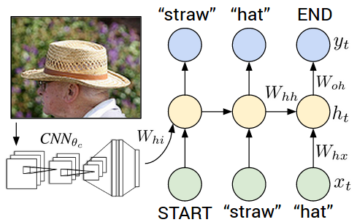
\includegraphics[width=0.5\linewidth]{Images/karpathy.PNG}
    \caption{Generatie van caption met recurrent neuraal netwerk}
\label{fig:rnntraining}
\end{figure}

Het trainen van het RNN gebeurt op basis van de Flickr30k dataset. 
Op basis van een willekeurig gekozen afbeelding uit de trainingsset berekent het netwerk de beste zin. Het verschil tussen deze voorspelling en de correcte zin propageert terug door het netwerk en leidt tot de juiste aanpassing van de gewichten

Wanneer de trainingsset volledig is doorlopen vindt een evaluatie plaats. De perplexity berekend op de resultaten voor de validatieset geeft snel aan of het netwerk nog bijleert of niet. Het systeem slaagt de tussentijdse resultaten op onder de vorm van checkpoints. Deze checkpoints bevatten alle nodige parameters om het opgeslagen model te evalueren. Er is ook de mogelijkheid om de training van het netwerk verder te zetten vanaf een bepaald checkpoint.

Formeel gezien berekent het netwerk op basis van input vectoren (woorden in de zin) $(x_1,x_2,...,x_T)$ een reeks van verborgen vectoren $(h_1,h_2,...,h_t)$. Deze verborgen vectoren dienen daarna als de basis voor output $(y_1,y_2,...,y_t)$. Deze outputs worden verkregen door formule \eqref{eq:rnn} te itereren voor $t = 1$ tot $T$.

\begin{equation}
\begin{aligned}
     b_v &= W_{hi} [CNN_{\theta_c}(I)] \\
     h_t &= f(W_{hx} x_{t} + W_{hh} h_{t-1} + b_h + \delta_{t1} \odot b_v) \\
     y_t &= softmax( W_{oh} h_t + b_o)
\end{aligned}
\label{eq:rnn}
\end{equation}
In deze vergelijkingen zijn $W_{hi}, W_{hx}, W_{hh}, W_{oh}$ en $b_h, b_o$ parameters die het netwerk leert. De $W_{xy}$ zijn gewichtsmatrices, terwijl $b_i$ bias vectoren zijn. $CNN_{\theta_c}(I)$ is de output van de laatste laag van VGGNet en $f$ is een activatiefunctie. $\delta_{t1}$ komt overeen met de Kroneckerdelta, die waarde $1$ heeft op tijdstip $t=1$. De output komt overeen met een kansverdeling over de verschillende woorden uit de dataset. Er is ook \'e\'en extra dimensie toegevoegd voor het END symbool dat het einde van een zin aangeeft. 

De code van Karpathy maakt ook op verschillende plaatsen gebruik van Rectified Linear Units of ReLu-encodering. Dit is een activatiefunctie die werkt volgens formule $ReLu(x) = max(x,0)$. De voornaamste reden hiervoor is effici\"entere gradientpropagatie. Het verlaagt het effect van verdwijnende gradi\"enten\cite{Glorot2011}. Er is ook de optie om te kiezen hoe groot de verborgen laag van het RNN moet zijn, alsook de optie om de afbeeldingsrepresentatie al dan niet tijdens elke stap toe te voegen.

Karpathy schrijft in zijn paper dat het eenmalig gebruiken van de afbeeldingsvector het beste resultaat geeft. Om dit te verifi\"eren hebben wij beide situaties vergeleken. Bij het gebruik van de afbeelding in elke stap verandert het tweede deel van formule \eqref{eq:rnn} in formule \eqref{eq:rnnfeedalways}.

\begin{equation}
     h_t = f(W_{hx} x_{t} + W_{hh} h_{t-1} + b_h + b_v)
\label{eq:rnnfeedalways}
\end{equation}

Het genereren van beschrijvingen gebeurt op basis van het beam search algoritme. Hierbij bepaalt de output van het netwerk de meest waarschijnlijke eerste woorden voor de zin. De beste $n$ woorden uit die ranking dienen dan als startpunt van de volgende iteratie. Op basis van deze woorden genereert het systeem alle mogelijke opeenvolgingen van twee woorden en voegt deze toe aan de lijst met zinnen bestaande uit \'e\'en woord. Het algoritme gaat door met de $n$ meest waarschijnlijke combinaties, die dus kunnen bestaan uit \'e\'en of twee woorden. Dit proces herhaalt zicht tot alle zinnen een END symbool voorspellen en dus volledig zijn, of tot een maximaal aantal iteraties bereikt is. 
 

\subsection{Long Short Term Memory Netwerk}
\label{sec:lstm}
De code van Karpathy werkt ook met een tweede type van neuraal netwerk. Dit netwerk volgt de methode van Vinyals et al.\cite{Google}. Het betreft een implementatie van een Long Short Term Memory neuraal netwerk. 

De gebruikte afbeeldingsrepresentatie is dezelfde als bij de RNN implementatie. We gebruiken de 4096-dimensionale feature vectors berekend met VGGNet. 

\paragraph{Van afbeelding naar beschrijving}
Anders dan het RNN van Karpathy, wordt de afbeeldingsrepresentatie beschouwd als het eerste woord in de zin. Ook de woordrepresentaties zijn dezelfde. Daarnaast gebruikt het een LSTM als taalmodel, een uitbreiding van een RNN. Op elk moment bevat het netwerk kennis over alle observaties tot op het huidige tijdstip. Door middel van \emph{gates} is er controle over het al dan niet onthouden van bepaalde waarden. Onderstaande vergelijkingen tonen de ontrolprocedure van het netwerk. Figuur \ref{fig:vinyals:karpathy} geeft een schematische weergave. Hierin is $x_t$ het $t+1^{de}$ woord van een zin en loopt $t$ van $0$ tot $N-1$. $W_{hi}$ transformeert de afbeeldingstransformatie naar een compactere codering. $LSTM$ in de gebruikte formule, staat samen met theoretische verduidelijking van het concept in sectie \ref{sub:lstm}. $p_{t+1}$ is de kansverdeling voor het $t+1^{de}$ woord van de gegenereerde zin.

\begin{eqnarray}
\vspace{-3mm}
x_{-1} = W_{hi}CNN(I)\\
p_{t+1} = LSTM(x_t)
\end{eqnarray}

\begin{figure}[tb]
	\centering
	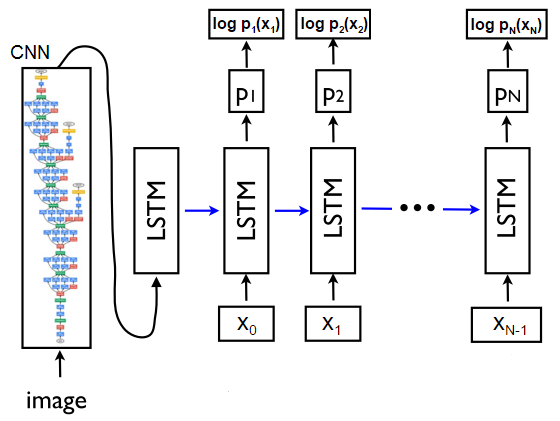
\includegraphics[width=1\linewidth]{Images/vinyals_karpathy.PNG}
	\caption{Ontrold LSTM-model}
	\label{fig:vinyals:karpathy}
\end{figure}

De training van het netwerk verloopt net als bij de RNN implementatie. Hierbij loop $t$ van $-1$ tot $N-1$ waarbij de afbeelding dus als woord $-1$ wordt beschouwd. Het netwerk leert op basis van de Flickr30k trainingsset en bij elke volledig doorlopen van de trainingsset berekenent de software de perplexity van de resultaten op de validatieset. Dit kan dienen als een criterium om de training stop te zetten. Voor een betere criterium verwijzen we naar hoofdstuk \ref{cha:experimenten}, dat de experimenten in detail beschrijft. %Verder in deze thesis beschrijven we een betere manier om te bepalen wanneer de training moet stoppen.\todo{laatste zin zou k anders doen}


Het genereren van nieuwe beschrijvingen voor ongeziene foto's gebeurt op exact dezelfde manier als bij RNN. Het ``beam search'' algoritme bepaalt de meest waarschijnlijke zin op basis van de uitkomst van het netwerk.


\section{Latent Dirichlet Analysis}
Het gebruik van Latent Dirichlet Analysis op een set van afbeeldingen en beschrijvingen heeft een groot voordeel in de taak van het genereren van nieuwe beschrijvingen. De onderwerpverdelingen bevatten extra semantische informatie die zeer bruikbaar kunnen zijn voor het genereren van beschrijvingen.

 Deze sectie beschrijft hoe LDA zorgt voor extra semantische informatie.

\subsubsection{Berekening van LDA-model}
\label{subs:Berekening van onderwerpverdeling}
Het leren van het gebruikte LDA model gebeurt op de Flickr30k dataset. Het algoritme om het LDA-model te bepalen beschouwt alle vijf beschrijvingen van een afbeelding achter elkaar als \'e\'en document. Net als in het voorbereiden van de data voor het taalmodel, houdt het enkel woorden over die meer dan vijf keer in de trainingsdata voorkomen. Vervolgens verwijdert het bovendien stopwoorden en stemt de woorden met behulp van een Porter stemmer. Beide voorbereidingstechnieken werden ge\"implementeerd met hulpmiddelen uit NLTK\footnote{http://www.nltk.org/}.

Het doel van het LDA-model is om op basis van een document, te bepalen welke onderwerps het sterkst aanwezig zijn. Het idee hierachter is dat een onderwerpverdeling ervoor kan zorgen dat het systeem woorden genereert die binnen het juiste onderwerp passen.

Het leren van dit model gebeurt met de python-bibliotheek \texttt{lda}\footnote{https://pypi.python.org/pypi/lda} en werkt intern met Gibbs sampling.

LDA heeft het aantal onderwerps als belangrijke parameter. Het evalueren van een LDA-model is een niet-triviale en moeilijk te automatiseren taak. Om die reden is het bepalen van het beste aantal onderwerps niet eenvoudig. Enkel indirecte evaluatie biedt de mogelijkheid om de prestatie van LDA indirect te bepalen. Jin et al.\cite{Jin2015} gebruiken ook LDA op dezelfde dataset en gebruiken 80 als aantal onderwerps. Daarom beschouwen we aantallen van onderwerps rond dit getal. 
Om toch een idee te krijgen van hoe het model presteert gaan we als volgt te werk. Eerst bepaalt een script per onderwerp de tien belangrijkste woorden. Op basis van deze woorden krijgt elk onderwerp een onderwerpnaam dat een overkoepelend concept voorstelt. 
Hierdoor is het enerzijds mogelijk om te kijken of de belangrijkste woorden in een onderwerp, een duidelijke link hebben. Anderzijds is het nu mogelijk voor elke afbeelding in de trainingsset de vijf belangrijkste onderwerpnamen op te vragen. Een manuele evaluatie van de onderwerps per afbeelding geeft opnieuw een idee over de prestatie van het LDA-model. Een voorbeeld van een trainingsafbeelding met de meest waarschijnlijke onderwerps is te zien in figuur \ref{fig:ldaonderwerps}. Voor extra voorbeelden verwijzen we naar appendix \ref{app:LDA}.

\begin{figure}[h]
	\centering
	\begin{minipage}[t]{.5\linewidth}
		\centering
		\vspace{0pt}
		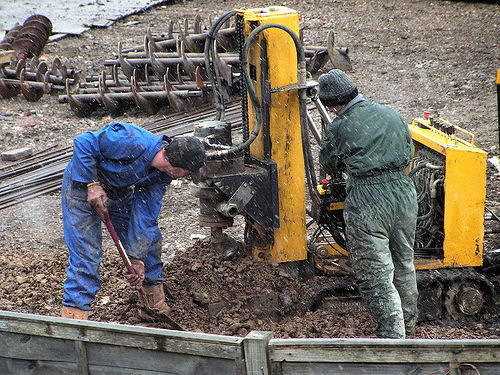
\includegraphics[width=\textwidth]{Images/LDA/5402085.jpg}
	\end{minipage}\hfill
	\begin{minipage}[t]{.5\textwidth}
		\centering
		\vspace{0pt}
		\begin{tabular}{ll}
			onderwerp                           & waarschijnlijkheid\\
			\hline
			\texttt{constuctor}             & 0.158 \\
			\texttt{work}                   & 0.113 \\
			\texttt{ground}                 & 0.113 \\
			\texttt{men together}           & 0.113 \\
			\texttt{work/metal/wood}        & 0.047\\
			\hline
		\end{tabular}
	\end{minipage}
	\caption{Voorbeeldfoto met de vijf meest waarschijnlijke onderwerpen}
	\label{fig:ldatopics}
\end{figure}

\subsubsection{Leren van netwerk}
\label{sec:LDAprediction}
Bij input van een nieuwe, ongeziene afbeelding moet het systeem in staat zijn om een onderwerpverdeling af te leiden. De beschrijvingen van de ongeziene afbeelding zijn niet gekend dus het LDA-model kan niet rechtstreeks worden gebruikt. Daarom is er een link nodig tussen een afbeeldingsrepresentatie en een onderwerpverdeling. Hiervoor zorgt een simpel feed-forward neuraal netwerk. 
Het netwerk zorgt voor de mapping van een afbeelding naar een onderwerpverdeling.

De trainingsverzameling in combinatie met de gekende onderwerpverdeling vormt de trainingsdata voor dit netwerk. 
Het geleerde LDA-model bepaalt vervolgens de onderwerpverdeling voor de zinnen in de validatieset. Deze onderwerp-verdelingen vormt de testverzameling voor het LDA-netwerk. Het doel van het trainen van het netwerk is de fout tussen de voorspelde verdeling en de berekende verdeling van de validatieverzamelingte verkleinen. De uiteindelijke fout van het finale netwerk maakt het mogelijk om verschillende configuraties te vergelijken.

Het gebruikte netwerk bestaat uit een inputlaag, een verborgen laag met 256 knopen en een outputlaag. De verborgen laag gebruikt de sigmo\"idefunctie \eqref{eq:sigmoid} als transferfunctie, terwijl de outputlaag een softmaxfunctie gebruikt, zoals uitgelegd in sectie \ref{par:softmax}. Experimenteel vormde de leersnelheid 0.001 de beste compromis tussen resultaat en snelheid van het leren.
Door middel van terugpropagatie leert het netwerk langzaamaan de gewichten. Dit netwerk kan op het moment van testen zeer snel een onderwerpverdeling bepalen voor een ongeziene afbeelding. Implementatie van het netwerk gebeurde met de python-bibliotheek \texttt{scikit-neuralnetwork}\footnote{https://scikit-neuralnetwork.readthedocs.org/en/latest/}
\begin{equation}
\sigma(t) = \frac{1}{1 + e^{-t}}
\label{eq:sigmoid}
\end{equation}

Wanneer het systeem een ongeziene afbeelding krijgt, gebeurt het volgende: VGGNet zet de afbeelding om naar een vectorrepresentatie. Deze vector dient als input voor de verborgen laag van het neuraal netwerk. Daarna transformeert de softmaxfunctie de output van de verborgen laag naar een kansverdeling over de verschillende onderwerps. Dit proces is ge\"illustreerd in figuur \ref{fig:learningLDA}.


\begin{figure}[tb]
    \centering
    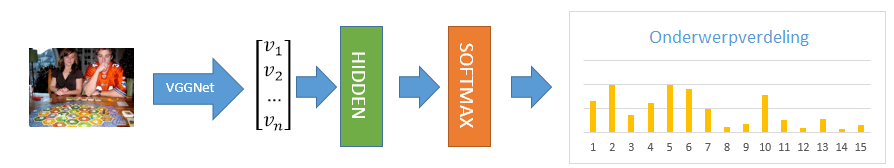
\includegraphics[width=\linewidth]{Images/LDANetwerk.PNG}
    \caption{Het proces om een ongeziene afbeelding te transformeren naar een onderwerpverdeling}
    \label{fig:learningLDA}
\end{figure}

Na het afronden van het trainingsproces zou het netwerk in staat moeten zijn om voor ongeziene afbeeldingen de bijhorende onderwerpsverdeling te genereren. Dit voorspelde resultaat komt meestal zeer goed overeen met de inhoud van de foto, figuur \ref{fig:ldalearningexample}. In uitzonderlijke gevallen zijn de voorspellingen allesbehalve correct, zoals in figuur \ref{fig:wrongldalearning}. Bij dit voorbeeld is wel duidelijk te zien dat er geen onderwerp is met een grote kans. Bij de correcte voorspelling is er meestal een onderwerp dat een veel grotere waarschijnlijkheid heeft dan de andere onderwerps. Meer voorbeelden van correcte en incorrecte voorspellingen zijn te vinden in appendix \ref{app:LDApredictions}.

\begin{figure}[h]
    \centering
    \begin{minipage}[t]{.5\linewidth}
    \centering
    \vspace{0pt}
    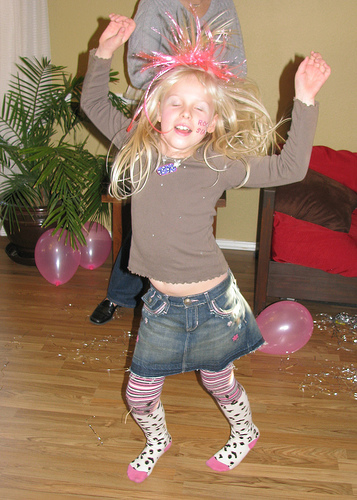
\includegraphics[width=\textwidth]{Images/LDA/2282260240.jpg}
    \end{minipage}\hfill
    \begin{minipage}[t]{.5\textwidth}
    \centering
    \vspace{0pt}
    \begin{tabular}{cl}
            onderwerp                           & waarschijnlijkheid\\
            \hline
            \texttt{girl}             & 0.235 \\
            \texttt{dance/perform}                   & 0.096 \\
            \texttt{playground}                 & 0.060 \\
            \begin{tabular}{c}
                \texttt{balloon/}\\
                \texttt{stuffed animal}
            \end{tabular}          & 0.041 \\
            \texttt{children}        & 0.034\\
            \hline
        \end{tabular}
    \end{minipage}
    \caption{Foto met de vijf meest waarschijnlijke onderwerps -- correcte voorspelling}
    \label{fig:ldalearningexample}
\end{figure}

\begin{figure}[h]
    \centering
    \begin{minipage}[t]{.5\linewidth}
    \centering
    \vspace{0pt}
    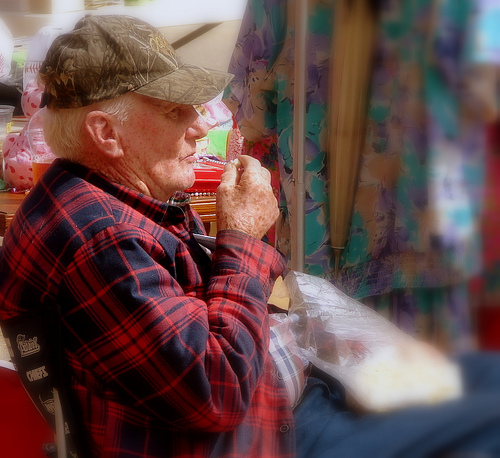
\includegraphics[width=\textwidth]{Images/LDA/3867804763.jpg}
    \end{minipage}\hfill
    \begin{minipage}[t]{.5\textwidth}
    \centering
    \vspace{0pt}
    \begin{tabular}{cl}
            onderwerp                           & waarschijnlijkheid\\
            \hline
            \texttt{musicians}             & 0.039 \\
            \texttt{work}                   & 0.037 \\
            \texttt{baby/toddler}                 & 0.031 \\
            \texttt{clothing}           & 0.027 \\
            \texttt{playground}        & 0.023\\
            \hline
        \end{tabular}
    \end{minipage}
    \caption{Foto met de vijf meest waarschijnlijke onderwerps -- incorrecte voorspelling}
    \label{fig:wrongldalearning}
\end{figure}


\section{Flickr30k Entities}
De dataset \emph{Flickr30k Entities}\cite{Plummer2015} is gebaseerd op de Flickr30k dataset. Ze bevat een groot aantal annotaties en omspannende rechthoek, alsook links tussen beide. Deze links kunnen een bron zijn van extra informatie. In deze sectie beschrijven we deze dataset in meer detail. Vervolgens volgt een bespreking van de pogingen om deze grote hoeveelheid informatie te verwerken naar een handelbaar formaat. 

\subsection{Dataset}
\label{sub:Dataset}
Flickr30k Entities is ontstaan op basis van een eenvoudig idee. De makers zien in dat een ``standaard'' afbeeldingsbeschrijvend systeem een globaal verband leert tussen een foto en een zin, zonder echt rekening te houden met de overeenkomsten tussen entiteiten op de foto en in de zin. Er zijn vrij recent wel een aantal systemen ontwikkeld die een mapping maken van afbeeldingsregio's naar beschrijvingen. Deze systemen veronderstellen echter dat deze verbanden latent zijn. Hier probeert de nieuwe Entities dataset verandering in te brengen, door de verbanden tussen beschrijving en foto te expliciteren.

De dataset is gebaseerd op de meer dan 30,000 afbeeldingen uit de Flickr30k dataset\cite{Young2014} met de bijhorende beschrijvingen. De makers brengen een uitbreiding hiervan, met een set van bijna 250,000 coreference chains, die verbanden aangeven tussen regio's uit de afbeeldingen en zinsdelen uit de beschrijvingen. Deze aanpak lijkt op wat de MS COCO\cite{Lin2014} dataset biedt, maar de objecten in de COCO dataset zijn onafhankelijk van de beschrijvingen gedetecteerd. Figuur \ref{fig:entities} toont een aantal voorbeelden van annotaties en references uit de Entities dataset, terwijl figuur \ref{fig:cocoexamples} toont hoe de verschillende objecten in de COCO dataset worden opgeslagen. Het is duidelijk dat er bij de COCO dataset geen rechtstreeks verband is met de beschrijvingen. 

\begin{figure}[!tb]
    \centering
    \begin{tabular}[t]{cc}
      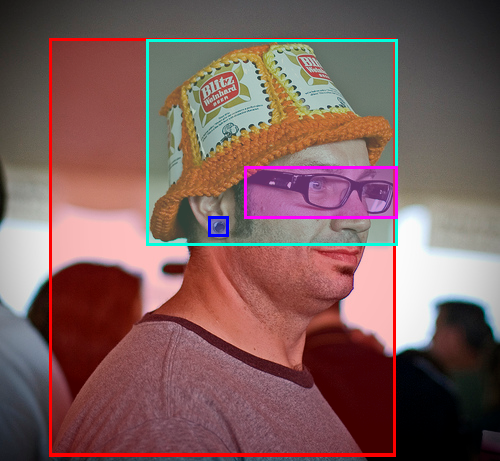
\includegraphics[height=3.0in]{Images/example_hat.png} \vspace{-3mm}&
      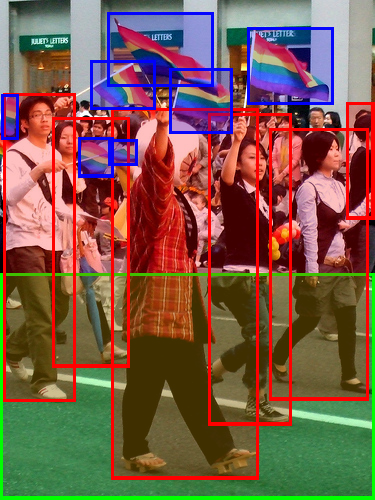
\includegraphics[height=3.0in]{Images/example_parade.png}\\
      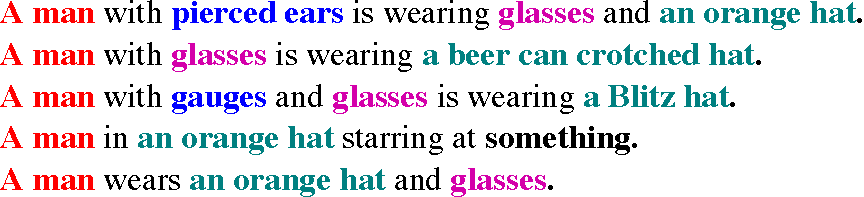
\includegraphics[valign = T,width=.4\columnwidth]{Images/example_hat_text.pdf}&
      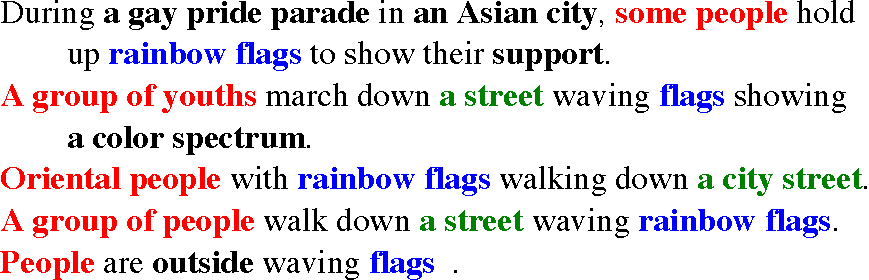
\includegraphics[valign = T,width=.4\columnwidth]{Images/example_parade_text.pdf}
  \end{tabular}
\caption{Voorbeelden van Flickr30k Entities annotaties. De kleur van de frases is overeenkomstig de kleur van de omspannende rechthoeken op de afbeelding\cite{Plummer2015}.}
\label{fig:entities}
\end{figure}

\begin{figure}
    \centering
    \subfloat{
        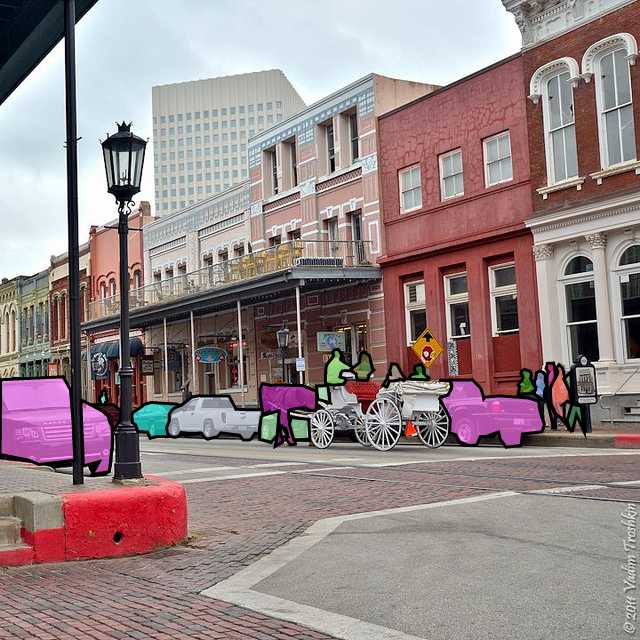
\includegraphics[width=0.47\linewidth]{Images/coco_example1.png}}\hfill
    \subfloat{
        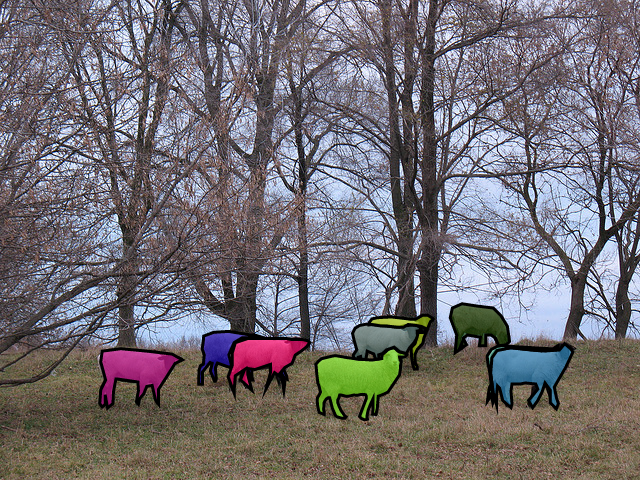
\includegraphics[width=0.47\linewidth]{Images/coco_example2.png}}
    \caption{Voorbeelden van geannoteerde afbeeldingen uit MS COCO dataset. Elk gekleurd object behoort tot \'e\'en van de objectcategorie\"en gedefinieerd door de makers.}
    \label{fig:cocoexamples}
\end{figure}

\subsection{Nut}
Flickr30k Entities vormt een dataset die een grote bron aan informatie bevat. Zo weet het direct waar in de afbeelding een woord of woordverzameling naar verwijst. Een netwerk dat deze informatie als extra input heeft, kan hieruit misschien extra informatie leren over bijvoorbeeld de grootte of locatie van bepaalde woorden in de afbeelding. Het kan ook een verrijking zijn voor bijvoorbeeld het ontdekken van ruimtelijke relaties. Daarnaast verwijzen meerdere formulaties soms naar dezelfde omspannende rechthoek. Het is dus mogelijk dat het netwerk semantisch gelijkaardige woorden zoals \texttt{huis} en \texttt{gebouw} als zodanig gaat beschouwen.


\subsection{Gebruik}
\label{sub:Gebruik}
Deze dataset bevat zeer veel extra informatie verspreid over een grote hoeveelheid verwijzingen. Een probleem dat zich voordoet is dat sommige van de omgevende rechthoeken zo klein zijn dat er amper informatie uit te halen is. Daarom is er een reductie uitgevoerd van de dataset alvorens over te gaan tot het verwerken van de data. 

Deze reductie gebeurt op basis van de grootte van de rechthoek. Een deel van de rechthoeken zijn slechts enkele pixels hoog of breed, waardoor een CNN hier weinig informatie kan uithalen. Deze te kleine rechthoeken worden daarom uit de dataset verwijderd. De limiet van zichtbaarheid en informatief zijn van een afbeelding staat ter discussie, maar wij kozen om alles kleiner dan 64 bij 64 pixels te verwijderen, wat resulteerde in 190,000 te gebruiken omspannende rechthoeken en corresponderende frases. 

De dataset is beschikbaar als tekstbestanden die weergeven welke omspannende rechthoeken op welke afbeelding te zien zijn, en met welke delen van de beschrijving elke box overeenkomt. Er zijn een aantal rechthoeken die wel zijn opgenomen in de dataset, maar geen overeenkomstig zinsdeel hebben. De semantische meerwaarde van dergelijke rechthoeken is miniem, dus horen deze ook niet tot de bekeken verzameling. 

Om de data bruikbaar te maken voor verwerking leest een script de tekstbestanden uit, en slaat alle rechthoeken op als aparte afbeelding. Op basis van die afbeeldingen berekent de Caffe-implementatie van VGGNet een vectorrepresentatie. De overeenkomstige zinsdelen zijn omgezet naar een tf-idf gewogen vectorweergave. Deze voorstelling is gebaseerd op twee belangrijke principes. Ten eerste is het gewicht van een woord in een zin proportioneel met het aantal keer dat het woord $i$ voorkomt in het document $j$ (term frequentie of $tf_{i,j}$). Ten tweede is het gewicht invers gerelateerd aan het aantal documenten $n_i$ waar het in voorkomt (inverse document frequentie of $idf_i$). Een woord dat in alle documenten voorkomt dient een lager gewicht te krijgen dan een woord dat slechts in een fractie van de documenten voorkomt. Formule \ref{formule:tfidf} toont het uiteindelijke resultaat. Het totaal aantal verschillende woorden is hier $N$\cite{Jurafsky:2009:SLP:1214993}. 

\begin{equation}
\label{formule:tfidf}
	tfidf_{i,j} = tf_{i,j}\cdot{idf_{i}} = tf_{i,j}\cdot{log(\frac{N}{n_i})}
\end{equation}

Op basis van de CCA-uitbreiding beschreven in sectie \ref{sub:stackedcca} berekenen we een uitgebreide representatie van de afbeeldingen uit de Flickr30k dataset. De extra informatie uit de overeenkomsten tussen omspannende rechthoeken en frasen zit vervat in een eerste gemeenschappelijke CCA ruimte. Uit de methodes voorgesteld door Gong et al.\cite{Gong2014} volgt een representatie van de trainingsafbeeldingen. Hierin is ook de informatie uit de Entities dataset aanwezig.

Het berekenen van de CCA mapping tussen de recthoeken en de frasen uit de Entities dataset verliep zonder problemen. De berekening van de augmentatie was ook probleemloos, maar tijdens het berekenen van de CCA mapping tussen de augmentaties van de Flickr30k foto's en hun beschrijvingen zijn we tot de conclusie gekomen dat het, door de hoge dimensionaliteit, qua tijdsbestek onhaalbaar was om deze mapping te gebruiken in onze experimenten. 



\section{Canonical Correlation Analysis}
Het toevoegen van extra semantische informatie kan gebeuren op verschillende manieren. Een eerste optie is LDA, zoals eerder beschreven. Er kan echter ook gebruik gemaakt worden van CCA. Waar LDA focust op het blootleggen van verbanden tussen de woorden uit de beschrijvingen, berekent CCA een ruimte die tussen de afbeelding en de zin ligt.

Het berekenen van deze tussenliggende ruimte gebeurt in twee stappen. Het eerder vernoemde VGGNet berekent de afbeeldingsvectoren voor de trainingsset. Een door tf-idf gewogen vector stelt de bijhorende zinnen voor, zoals eerder beschreven. 

Belangrijk is dat alle zinnen apart worden beschouwd. Waar bij LDA de vijf zinnen per afbeelding worden gereduceerd tot \'e\'en zin, blijven ze hier apart. Dit om ervoor te zorgen dat de mapping rekening houdt met de verschillende zinnen, moest er sprake zijn van heel verschillende formuleringen van dezelfde concepten. Meer concreet houdt dit in dat elke foto maximaal gecorreleerd dient te zijn met vijf verschillende zinnen uit de trainingsset. 

Een deel van de rijkdom van de dataset gaat verloren als er gebruikt wordt gemaakt van een aaneensluiting van de verschillende zinnen. Bij LDA doet dit probleem zich niet voor, en is het zelfs beter om de zinnen bij elkaar te voegen, aangezien we \'e\'en onderwerpverdeling per afbeelding beogen, en niet per zin. Synoniemen en afgeleiden worden beschouwd als deel van hetzelfde document, juist door de aaneensluiting van de zinnen.

Na het berekenen van de representaties van afbeeldingen en zinnen volgt een berekening van de correlatiecomponenten. Dit gebeurt met de \texttt{MATLAB}-implementatie van het canonical correlation algoritme. Het resultaat bestaat uit twee projectiematrices, die dienen om afbeeldings- en beschrijvingsvectoren te projecteren op de tussenliggende ruimte die de correlatie maximaliseert. Voor onze experimenten maken we enkel gebruik van de projectie voor afbeeldingen, aangezien Jia et al.\cite{Fernando2015} aantonen dat het gebruik van enkel de afbeeldingsprojectie de beste resultaten oplevert.


\section{Toevoeging van LDA onderwerpverdeling aan RNN}
De eerder berekende onderwerpverdelingen kunnen dienen als extra semantische informatie om de generatie in de juiste richting te sturen. Het integreren van de onderwerpverdeling $L$ in het RNN gebeurt volgens formule \eqref{eq:rnnldaonce} die het tweede deel van \eqref{eq:rnn} vervangt. Het rode deel in de formule duidt de verschillen met \eqref{eq:rnn} aan. $W_l$ is een gewichtsmatrix voor vermenigvuldiging met de onderwerpverdeling.

\begin{equation}
    h_t = f(W_{hx} x_{t} + W_{hh} h_{t-1} + b_h + \mathbbm{1}{(t=1)} \odot b_v +\color{red}{\mathbbm{1}{(t=1)} \odot W_lL}
    \color{black}
    \label{eq:rnnldaonce}
\end{equation}

Er kan ook gekozen worden om de onderwerpverdeling elke stap toe te voegen, wat leidt tot formule \eqref{eq:rnnldaall}. Het lijkt ons interessant om te experimenteren met het al dan niet altijd toevoegen van de onderwerp informatie. Dit kan, in tegenstelling tot het steeds toevoegen van de afbeelding, een verbetering betekenen. De informatie uit de onderwerpverdeling is afgeleid van de afbeelding, maar bevat informatie van een lagere dimensionaliteit. Het herhaaldelijk meegeven van de onderwerp vector zorgt dat het netwerk elke stap deze semantische informatie binnenkrijgt. Voor een gedetailleerde beschrijving van de uitgevoerde experimenten, en een vergelijking tussen de verschillende settings verwijzen we u door naar hoofstuk \ref{cha:resultaten}.


\begin{equation}
    h_t = f(W_{hx} x_{t} + W_{hh} h_{t-1} + b_h + \mathbbm{1}{(t=1)} \odot b_v + W_lL
    \label{eq:rnnldaall}
\end{equation}


\section{gLSTM}
\subsection{Guided LSTM}
Guided Long Short Term Memory (gLSTM) is een recente uitbreiding van het LSTM model ge\"introduceerd door Jia et al.\cite{Fernando2015} In dit model extraheren ze eerst semantische informatie van elke afbeelding. Deze informatie dient dan als extra input of ``gids'' voor het LSTM-blok.

Na het bestuderen van bestaande LSTM-modellen ontdekten de auteurs dat de gegenereerde zinnen ``semantische drift'' vertonen. Dit wil zeggen dat naarmate de zin evolueert, de betekenis van volgende woorden steeds minder met de input-afbeelding te maken heeft. Ze vermoeden dat dit komt door twee tegenwerkende krachten. Enerzijds moet de zin de afbeelding beschrijven, anderzijds moet de zin passen in het taalmodel. Om die reden introduceren ze een semantische gids, die ervoor moet zorgen dat het model na enkele woorden op het juiste pad blijft. Dit gebeurt door aan woorden die semantisch verbonden zijn aan de afbeelding een positieve bias te geven.

Ze gebruiken vier verschillende semantische gidsen in hun experimenten. Als eerste model gebruiken ze een ``retrieval-based'' gids. Hierbij zoeken ze eerst naar zinnen die gerelateerd zijn aan de afbeelding. Vervolgens verzamelen ze daaruit de zinnen met de hoogste rang. Deze zinnen vormen dan de extra input.
Als tweede model leren ze eerst een CCA-model. Vervolgens nemen de auteurs de projectie van de afbeeldingsrepresentatie in de gemeenschappelijke ruimte. Daarna worden de dichtstbijzijnde geprojecteerde zinnen gezocht op basis van cosinusgelijkheid. Ook hier vormen de hoogst scorende zinnen de extra input.
Een derde model gebruikt de CCA-projectie van de afbeelding in de gemeenschappelijke ruimte rechtstreeks als gids.
Als laatste model gebruiken ze de afbeeldingsrepresentatie zelf als gids.

Om dit te implementeren starten ze net als in deze masterproef van de LSTM-implementatie van Karpathy. Ze defin\"ieren de geheugencellen en poorten zoals in de volgende formules. Hierbij zijn de rode delen toevoegingen ten opzichte van de standaard LSTM \ref{lstm-memory-start}-\ref{lstm-memory}:

%
\begin{eqnarray}
\vspace{-3mm}
\label{glstm-memory-start}
i_l' & = & \sigma (W_{ix} x_l + W_{im} m_{l-1} \color{red}{+ W_{iq} g}) \label{glstm-input} \\
f_l' & = & \sigma (W_{fx} x_l + W_{fm} m_{l-1} \color{red}{+ W_{fq} g}) \\
o_l' & = & \sigma (W_{ox} x_l + W_{om} m_{l-1} \color{red}{+ W_{oq} g}) \\
c_l' & = & f_l' \odot c_{l-1}' + i_l' \odot h(W_{cx} x_l + \nonumber \\
&   & + W_{cm} m_{l-1} \color{red}{+ W_{cq} g}) \\
m_l & = & o_l' \odot c_l'
\label{glstm-memory}
\vspace{-3mm}
\end{eqnarray}
Hierbij is $g$ de vectorvoorstelling van de semantische informatie. De gids is onafhankelijk van de tijdstap en werkt dus globaal voor elke afbeelding. $W_{iq}$, $W_{fq}$, $W_{oq}$ en $W_{cq}$ zijn extra gewichtsmatrices die het netwerk in de trainingsfase moet leren. Figuur \ref{fig:glstm} geeft een visuele voorstelling van de gLSTM-blok.

\begin{figure}[tb][h]
	\centering
	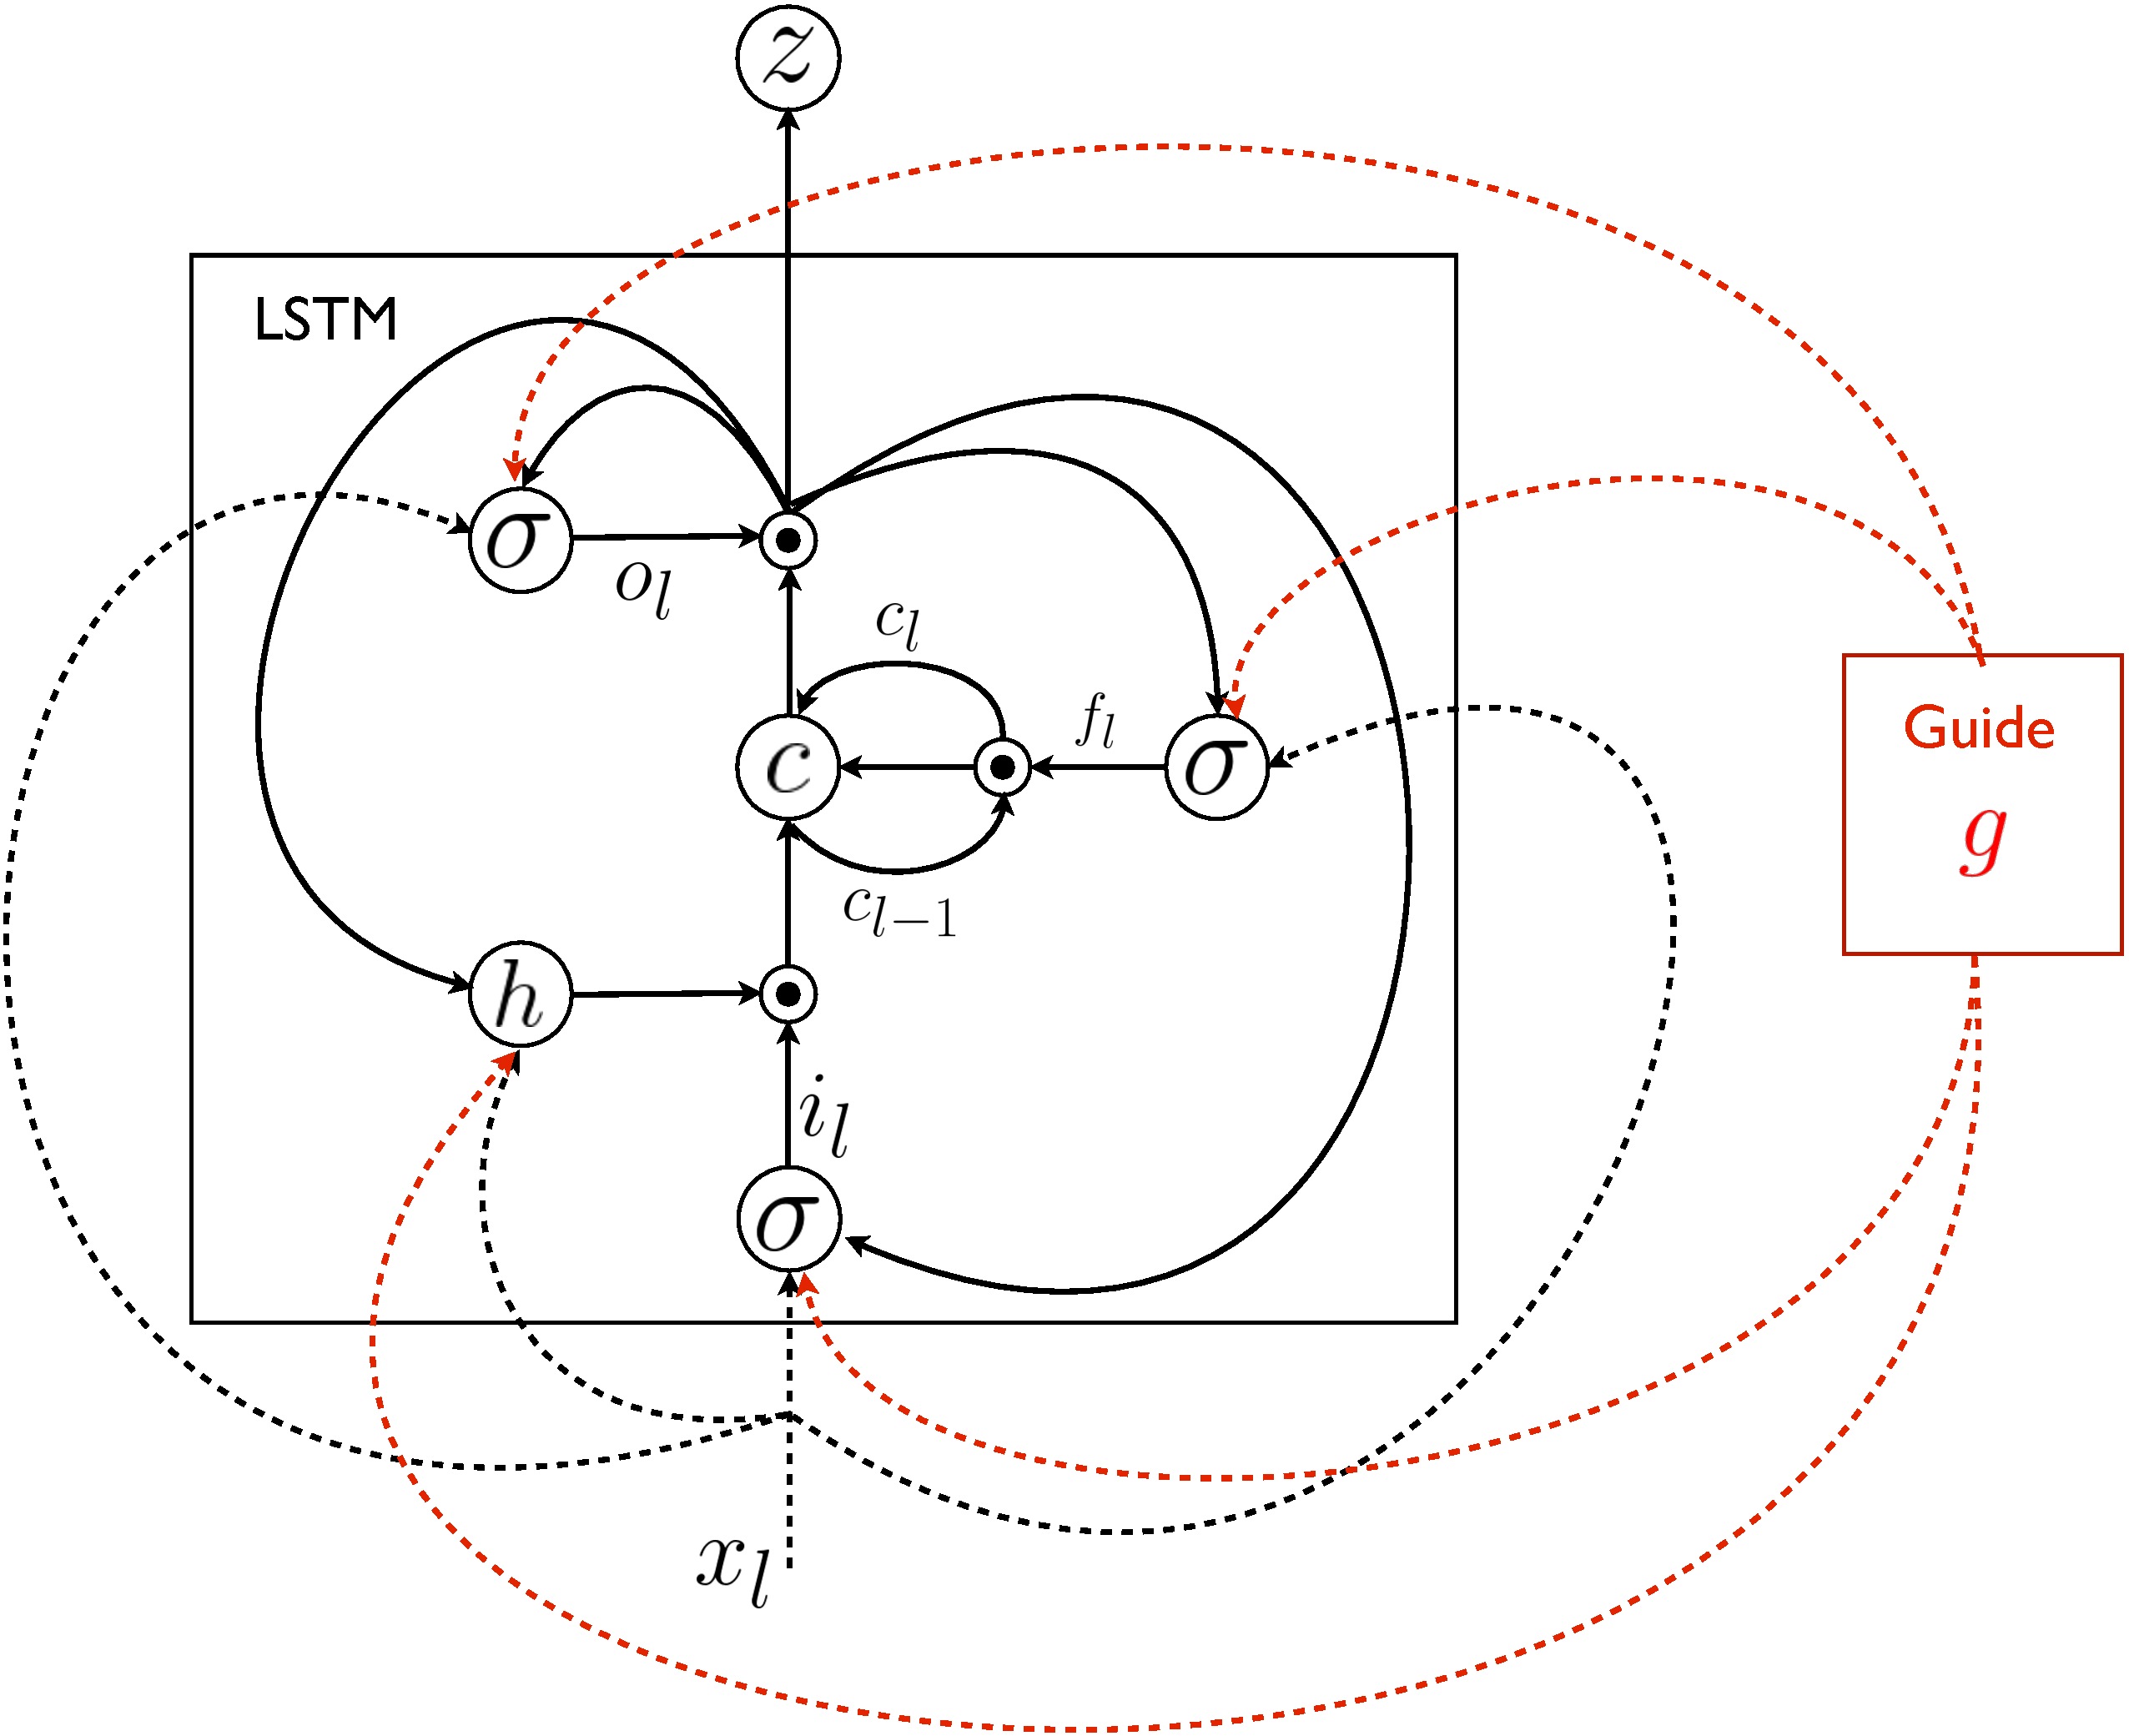
\includegraphics[width=\linewidth]{Images/glstm.pdf}
	\caption{LSTM-blok in het zwart. Uitbreidingen van gLSTM in het rood.}
	\label{fig:glstm}
\end{figure}

Jia et al. bekomen zeer goede resultaten. De eerste drie gidsen zorgen voor verbetering op hun baseline. Enkel de afbeelding als gids zorgt voor verslechtering. De rechtstreekse CCA-projectie presteert het beste.

\subsection{gLSTM met LDA en CCA}
Net als Jia implementeren we de gLSTM als een uitbreiding van LSTM overeenstemmend met formules \ref{glstm-memory-start}-\ref{glstm-memory}.
Om te kunnen vergelijken met hun paper kan de implementatie ook de CCA-projectie als gids gebruiken.
Daarnaast is een veronderstelling dat LDA een goede bron van semantische informatie is. Het bevat immers een verdeling van de onderwerpen die aanwezig zijn in de afbeelding. Daarom kan LDA ook als gids worden gekozen.
We voorzien dus twee modellen zodat het mogelijk is om na te gaan wat de betere gids is in deze configuratie van de gLSTM.

\section{Normalisatie van beam search}
Naast het introduceren van gLSTM's breiden Jia et al.\cite{Fernando2015} de implementatie van Karpathy nog op een tweede manier uit. Na evaluatie van bestaande modellen leidden ze af dat het gebruikte beam-search algoritme een voorkeur heeft voor kortere zinnen. Beam-search neemt de som van de log-likelihood van individuele woorden als criterium. Aangezien deze waarde voor elk woord negatief is, zal het algoritme sneller kiezen om te stoppen dan nog een woord toe te voegen. Om dit fenomeen tegen te gaan introduceren ze de genormaliseerde log-likelihood van elk woord als criterium. Concreet betekent dit een extra normalisatiefactor $\Omega$ bij de berekening van de waarschijnlijkheid van een woordsequentie.

\begin{equation}
p = \frac{1}{\color{red}{\Omega(\ell)}}\sum_{l=1}^{\ell} \log p(s_l | im, s_{1:l}, \theta)
\label{eq:log-sentence-norm}
\end{equation}

In deze formule is $l$ de lengte van de huidige woordsequentie. $p$ stelt de waarschijnlijkheid voor. $s_i$ is het $i^{de}$ woord in de sequentie, $im$ de afbeelding en $\theta$ de parameters van het model. 

De auteurs van de paper bestuderen meerdere functies voor $\Omega$. Wij implementeren de twee meest performante.
Enerzijds gebruiken we de Gaussiaanse functie $\Omega(\ell) \sim \mathcal{N}(\mu, \sigma)$, waar $\mu$ en $\sigma$ respectievelijk het gemiddelde en de standaardafwijking zijn van de lengtes van de zinnen in het trainingscorpus. Hierdoor moeten gegenereerde zinnen gelijkaardige lengtes hebben aan deze uit het corpus. 
Anderzijds implementeren we de min-hinge normalisatie. Met deze methode is de normalisatiefactor gelijk aan de gemiddelde lengte van het trainingscorpus ($\mu$) als de zin langer is dan dit gemiddelde. Indien de zin korter is, is de factor gelijk aan de lengte van de zin. Dit komt overeen met de functie $\Omega(\ell)=\min\{\ell, \mu\}$.

Een eigen implementatie van de $\Omega(\ell)$ functie maakt gebruik van idf-gewichten. Deze gewichten zijn gebaseerd op het aantal afbeeldingen uit de trainingsverzameling waarbij het woord in kwestie voorkomt in \'e\'en van de vijf beschrijvingen. Alvorens deze gewichten te berekenen zijn de stopwoorden verwijderd uit de trainingszinnen en zijn alle woorden gereduceerd met een Porter stemming algoritme. De berekende gewichten ($idf_i$) voor elk woord ($w_i$) komen dan overeen met volgende formule: 

\begin{equation}
    idf_i = \log(\frac{N}{n_i})
\end{equation}
Hierbij stelt $N$ het aantal afbeeldingen voor en staat $n_i$ voor het aantal afbeeldingen waar het woord $w_i$ voorkomt in de beschrijvingen.

Deze gewichten vertonen een verband met de hoeveelheid informatie die het woord bevat. Voorbeelden van woorden met laagste en hoogste IDF staan respectievelijk in tabel \ref{tbl:idf-laag} en tabel \ref{tbl:idf-hoog}. Om een normalisatie te verkrijgen, telt het algoritme de gewichten voor alle afzonderlijke woorden op. Op deze manier is er een afstraffing voor zinnen die veel frequente woorden bevatten en dus zo minder veelzeggend zijn. Anderzijds zorgt dit er ook meteen voor dat korte zinnen niet langer de voorkeur krijgen.
\todo[inline]{IDF-norm moet ook stoppen als lengte te groot is -> da nog toevoegen als geimplementeerd}

\todo[inline]{deze captions zijn vreemd. alle, nu is er tabel 5.1, 5.2 en 5.3}
\begin{table}[!htb]
	\caption{Gestemde woorden samen met hun IDF-gewicht}
	\begin{minipage}{.5\linewidth}
		\caption{Woorden met laagste IDF}
		\label{tbl:idf-laag}
		\centering
		\begin{tabular}{ll}
    man    & 1.099 \\
    two    & 1.946 \\
    woman  & 1.946 \\
    people & 2.198 \\
    shirt  & 2.303 \\
		\end{tabular}
	\end{minipage}%
	\begin{minipage}{.5\linewidth}
		\centering
		\caption{Woorden met hoogste IDF}
		\label{tbl-idf-hoog}
		\begin{tabular}{ll}
	fingerless & 10.275\\
	creamer& 10.275\\
	vigor& 10.275\\
	ghetto& 10.275\\
	raceway& 10.275\\
		\end{tabular}
	\end{minipage} 
\end{table}

\todo[inline]{Dit updaten als we iets beter vinden}
Op basis van twee normalisatiefuncties hierboven beschreven is het mogelijk om een combinatie te maken. Het gebruik van zowel Gaussiaanse als idf-normalisatie zou kunnen leiden tot betere resultaten. Het idee hierachter is dat zowel korte zinnen als weinig informatieve zinnen een penalisatie ondervinden. Het berekenen van deze normalisatiefactor gebeurt door eerst de idf-gewichten van alle woorden in de zin op te tellen en deze som vervolgens te vermenigvuldigen met de waarde van de Gaussiaanse functie die hierboven is beschreven.

\section{FSMN}
E\'en van de eerste wijzigingen die we in deze thesis probeerden te implementeren, waren Feedforward Sequential Memory Neural Networks (FSMN)\cite{Zhang}. Deze netwerken vormen een uitbreiding op gewone feed-forward neurale netwerken. Dit netwerk kan afhankelijkheden op lange termijn leren zonder recurrente verbindingen te gebruiken. Het doet dit door sequenti\"ele geheugenblokken in de verborgen lagen van het feed-forward netwerk te steken. 

Volgens de paper zijn deze netwerken in staat om betere en vooral snellere resultaten te leveren dan de huidige RNN-modellen. De snellere resultaten zijn mogelijk omdat gebruik kan worden gemaakt van standaard terugpropagatie zonder dat er zich problemen voordoen door de recurrente verbindingen. Figuur \ref{fig:fsmn} toont de  algemene structuur van dit netwerk. Hierbij dient de output van een verborgen laag als input voor een geheugenblok. Dit geheugenblok is in staat om informatie bij te houden van meerdere vorige inputs. Het geheugenblok dient dan zelfs als extra invoer voor een volgende laag.

Vooral de snellere resultaten leken zeker een goede uitbreiding voor het model van Karpathy. Trainen van een RNN batch duurt immers ongeveer 4 seconden en voor LSTM 7 seconden. Hierdoor duurt het volledig trainen van het neuraal netwerk gemiddeld meer dan zeven dagen.
Hoewel de implementatie van dit netwerk op basis van de paper succesvol was, vertoonden de resultaten zowel qua kwaliteit en snelheid geen verbetering. Om die reden hebben we geen verdere experimenten met FSMN's uitgevoerd.

\begin{figure}[tb]
	\centering
	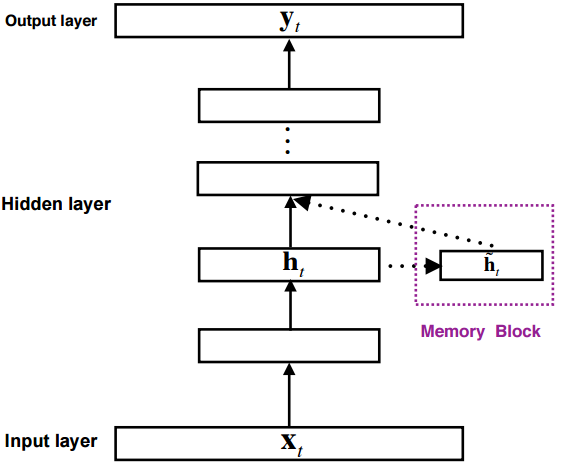
\includegraphics[width=0.6\linewidth]{Images/FSMN}
	\caption{Algemene structuur van Feedforward Sequentieel Geheugen Neural Netwerken.}
	\label{fig:fsmn}
\end{figure}
